% Made up for the tikra benchmark.
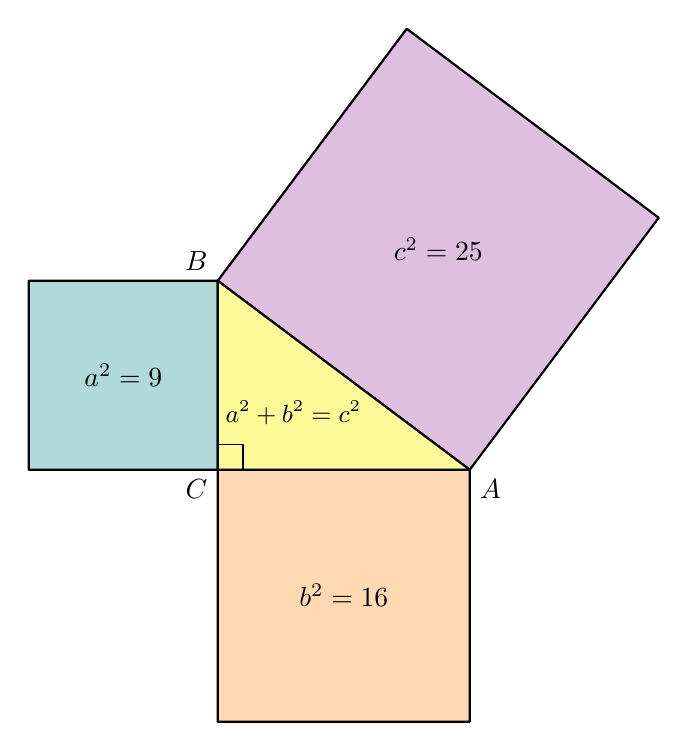
\begin{tikzpicture}[scale=0.8, line join=round, thick]
  % right triangle with legs 3 and 4, right angle at C
  \coordinate (C) at (0,0); \coordinate (A) at (4,0); \coordinate (B) at (0,3);
  \draw[fill=orange!30] (C) -- (A) -- (4,-4) -- (0,-4) -- cycle;
  \draw[fill=teal!30] (C) -- (B) -- (-3,3) -- (-3,0) -- cycle;
  \draw[fill=violet!25] (A) -- (B) -- (3,7) -- (7,4) -- cycle;
  \draw[fill=yellow!40] (C) -- (A) -- (B) -- cycle;
  \draw[thin] (0.4,0) -- (0.4,0.4) -- (0,0.4);
  \node at (2,-2) {$b^2 = 16$};
  \node at (-1.5,1.5) {$a^2 = 9$};
  \node at (3.5,3.5) {$c^2 = 25$};
  \node[font=\small] at (1.2,0.9) {$a^2+b^2=c^2$};
  \node[below left] at (C) {$C$};
  \node[below right] at (A) {$A$};
  \node[above left] at (B) {$B$};
\end{tikzpicture}
